\documentclass{beamer}

\RequirePackage{tikz}
\usetikzlibrary{shapes.misc}
\usetikzlibrary{positioning,intersections}
\usetikzlibrary{petri}
\usetikzlibrary{calc,intersections,through,backgrounds}
\usetikzlibrary{calc,decorations.pathmorphing,patterns}

\usepackage{alltt}
\usepackage{url}

\usetheme{PUT}
\title{Not-So-Linked Solution to the\\Linked Data Mining Challenge 2016}
\author{Jedrzej Potoniec}
\date{30.05.2016}
\institute{Institute of Computing Science, Poznan University of Technology}
\begin{document}
\begin{frame}
\titlepage
\end{frame}
\begin{frame}{Agenda}
\begin{enumerate}
\item Feature construction
\item Machine learning workflow
\item Insight into ML model
\item Short conclusion
\end{enumerate}
\end{frame}
%TODO irregularities?


%In the beginning, we planned to extract features from \emph{DBpedia} using \emph{Fr-ONT-Qu} \cite{frontqu} from \emph{RMonto} \cite{rmonto}, a plugin to \emph{RapidMiner} \cite{rapidminer}.
%Unfortunately, the most promising feature discovered this way was a binary information if an album has a review score from \emph{Pitchfork}\footnote{\url{http://pitchfork.com/}} or not.
%After investigating, we discovered that during the extraction from \emph{Wikipedia} to \emph{DBpedia} a relation between a reviewing website and a review score has been lost.
%Consider triples for the \emph{Strange Mercy} album\footnote{\url{http://dbpedia.org/page/Strange_Mercy}}: there are 11 triples with a property \texttt{dbp:rev} and a few triples with properties like \texttt{dbp:rev10score}, but one has absolutely no way to connect scores to the reviewing websites.
%The very same problem happens with properties \texttt{dbp:title} (12 values) and \texttt{dbp:length} (11 values): it is impossible to decide on a length for a concrete track.
%
%We thought about using \emph{Yago} \cite{yago}, but it seemed to lack review information.
%We also tried to use \emph{DBTune}\footnote{\url{http://dbtune.org/}}, as suggested by the challenge website, but it rendered out to be a dead end.
%For example, \emph{MusicBrainz data}, the most interesting dataset there, is a \emph{Service Temporarily Unavailable} for a very long time now.
\begin{frame}{Linked datasets: DBTune}
\begin{tikzpicture}
\node {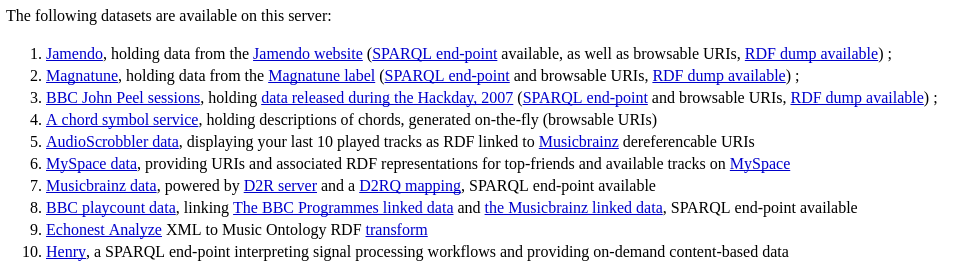
\includegraphics[scale=.6]{dbtune.png}};
\draw[thick,red,->] (-7.8,-.85) -- +(.5,0);
\end{tikzpicture}
\only<2->
{
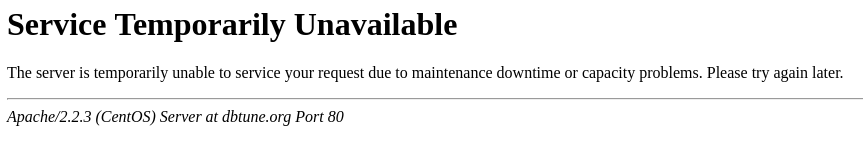
\includegraphics[width=\textwidth]{linkedbrainz.png}
}
\end{frame}

\begin{frame}{Linked datasets: DBpedia}
\url{https://en.wikipedia.org/wiki/Strange_Mercy?oldid=667760297}

\pause
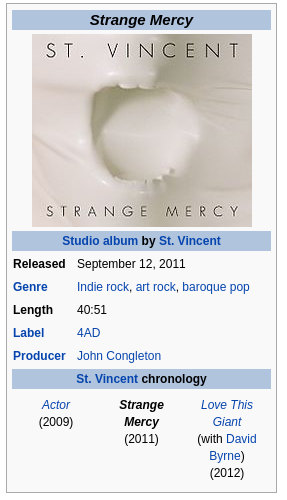
\includegraphics[width=.32\textwidth]{strange_mercy1.png}
\pause
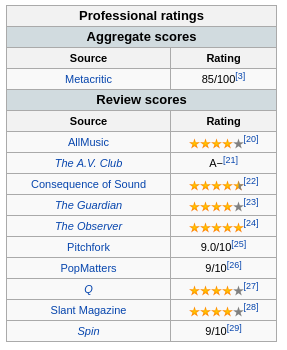
\includegraphics[width=.32\textwidth]{strange_mercy2.png}
\pause
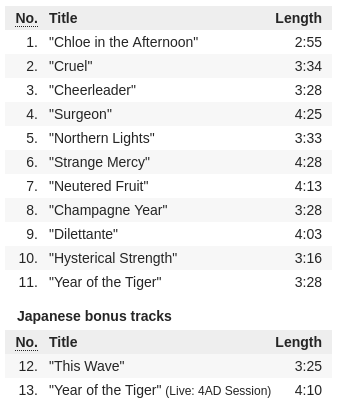
\includegraphics[width=.32\textwidth]{strange_mercy3.png}
\end{frame}

\begin{frame}{Linked datasets: DBpedia}
\url{http://dbpedia.org/resource/Strange_Mercy}
\vspace{.5cm}

\begin{tabular}{l|l}
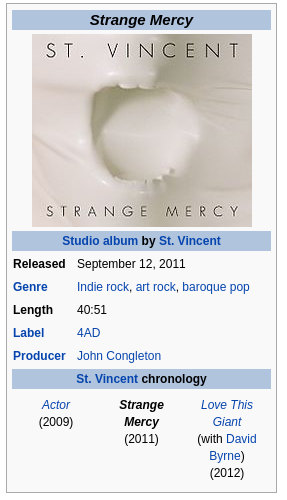
\includegraphics[width=.32\textwidth]{strange_mercy1.png}
&
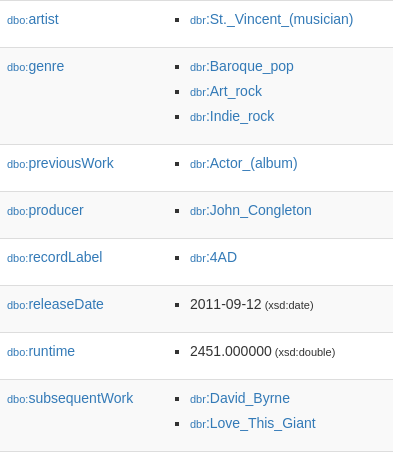
\includegraphics[width=.5\textwidth]{dbpedia1.png}
\end{tabular}
\end{frame}

\begin{frame}{Linked datasets: DBpedia}
\url{http://dbpedia.org/resource/Strange_Mercy}
\vspace{1cm}

\begin{tabular}{l|l}
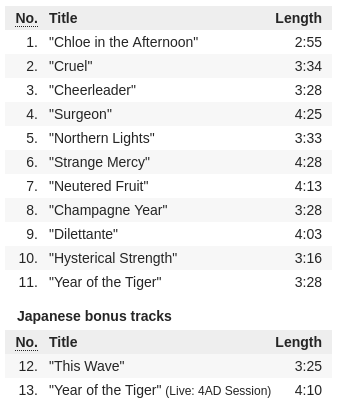
\includegraphics[width=.32\textwidth]{strange_mercy3.png}
&
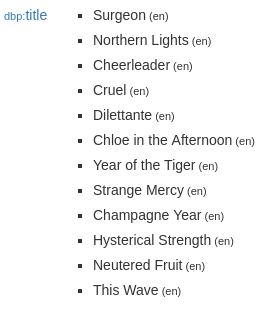
\includegraphics[width=.32\textwidth]{dbpedia3a.png}
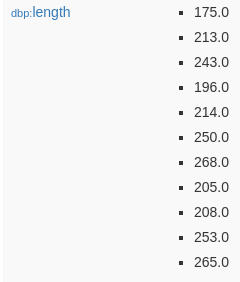
\includegraphics[width=.32\textwidth]{dbpedia3b.png}
\end{tabular}
\end{frame}

\begin{frame}{Linked datasets: DBpedia}
\url{http://dbpedia.org/resource/Strange_Mercy}
\vspace{1cm}

\begin{tabular}{l|l}
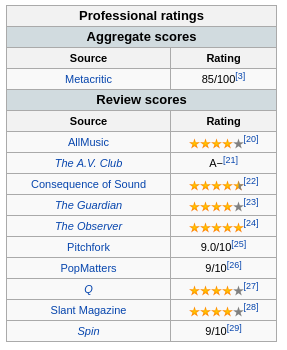
\includegraphics[width=.32\textwidth]{strange_mercy2.png}
&
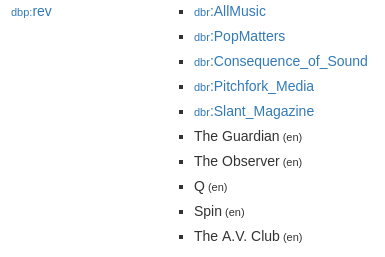
\includegraphics[width=.32\textwidth]{dbpedia2a.png}
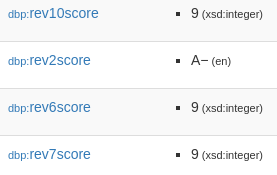
\includegraphics[width=.32\textwidth]{dbpedia2b.png}
\end{tabular}
\end{frame}

\begin{frame}{Non-linked datasets}
\centering

\includegraphics[width=\textwidth]{python-logo-master-v3-TM.png}

\centering

\includegraphics[width=\textwidth]{scrapy-logo.jpg}
\end{frame}

\begin{frame}[fragile]{Wikipedia}
\begin{verbatim}
{{album ratings
|MC=85/100<ref name=metacritic/>
| rev1       = [[AllMusic]]
| rev1Score  = {{rating|4|5}}<ref name=allmusic>Phares, Heather. [http://allmusic.com/album/strange-mercy-r2220859/review Strange Mercy&nbsp;– St. Vincent]. [[Allmusic]]. Retrieved 14 September 2011.</ref>
| rev2       = ''[[The A.V. Club]]''
| rev2Score  = A−<ref name=avclub>Adams, Erik. [http://www.avclub.com/articles/st-vincent-strange-mercy,61595/ St Vincent: Strange Mercy]. [[The A.V. Club]]. 13 September 2011. Retrieved 13 September 2011.</ref>
| rev3       = [[Consequence of Sound]]
| rev3Score  = {{rating|4.5|5}}<ref name=cos>Kivel, Adam. [http://consequenceofsound.net/2011/09/album-review-st-vincent-strange-mercy/ Album Review: St. Vincent – Strange Mercy]. [[Consequence of Sound]]. 9 September 2011. Retrieved 9 September 2011.</ref>
| rev4       = ''[[The Guardian]]''
| rev4Score  = {{rating|4|5}}<ref name=guardian>Nicholson, Rebecca. [http://www.guardian.co.uk/music/2011/sep/08/st-vincent-strange-mercy-review St Vincent: Strange Mercy – review]. [[The Guardian]]. 8 September 2011. Retrieved 8 September 2011.</ref>
| rev5       = ''[[The Observer]]''
| rev5Score  = {{rating|5|5}}<ref name=observer>Woodcraft, Molloy. [http://www.guardian.co.uk/music/2011/sep/11/st-vincent-strange-mercy-review St Vincent: Strange Mercy – review]. [[The Observer]]. 11 September 2011. Retrieved 12 September 2011.</ref>
| rev6       = [[Pitchfork Media|Pitchfork]]
| rev6Score  = 9.0/10<ref name=pitchfork/>
| rev7       = [[PopMatters]]
| rev7Score  = 9/10<ref name=popmatters>Pan, Arnold. [http://www.popmatters.com/pm/review/148401-st.-vincent-strange-mercy/ St. Vincent: Strange Mercy]. [[Popmatters]]. 12 September 2011. Retrieved September 2011.</ref>
| rev8       = ''[[Q (magazine)|Q]]''
| rev8Score  = {{rating|4|5}}<ref name="q"/>
| rev9       = [[Slant Magazine]]
| rev9Score  = {{rating|4|5}}<ref name=slant>Liedel, Kevin. [http://www.slantmagazine.com/music/review/st-vincent-strange-mercy/2616 St. Vincent: Strange Mercy]. [[Slant Magazine]]. 12 September 2011. Retrieved 12 September 2011.</ref>
| rev10      = ''[[Spin (magazine)|Spin]]''
| rev10Score = 9/10<ref name=spin>Anderson, Stacey. [http://www.spin.com/reviews/st-vincent-strange-mercy-4ad St. Vincent 'Strange Mercy']. [[Spin (magazine)|Spin]]. Retrieved 7 September 2011.</ref>
}}
\end{verbatim}
\end{frame}

\begin{frame}{Musicbrainz}
\centering
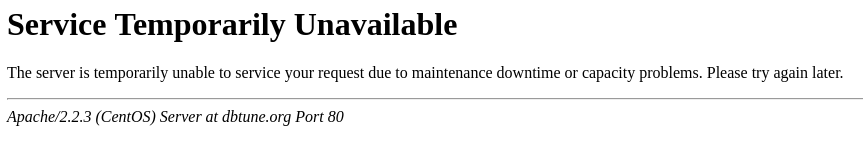
\includegraphics[width=\textwidth]{musicbrainz.png}
\end{frame}

\begin{frame}{Discogs}
\centering
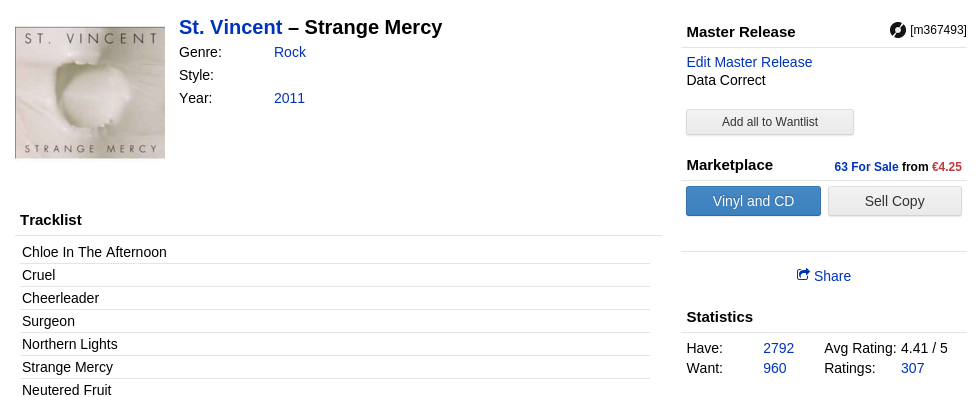
\includegraphics[width=\textwidth]{discogs.png}
\end{frame}

\begin{frame}{Amazon}
\centering
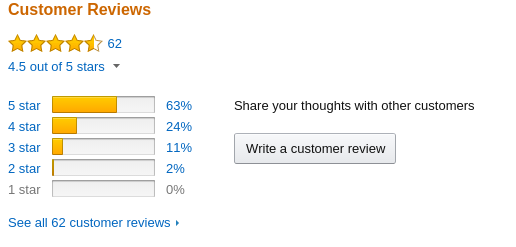
\includegraphics[width=\textwidth]{amazon.png}
\end{frame}

\begin{frame}{Non-linked dataset}
\begin{itemize}
\item RDF
\url{github.com/jpotoniec/LDMC2016/blob/master/data.ttl}
\item CSV
\begin{itemize}
\item \url{github.com/jpotoniec/LDMC2016/blob/master/wikiscraper/reviews.csv}
\item \url{github.com/jpotoniec/LDMC2016/blob/master/musicbrainz/ratings.csv}
\item \url{github.com/jpotoniec/LDMC2016/blob/master/discogs/discogs.csv}
\item \url{github.com/jpotoniec/LDMC2016/blob/master/amazon/amazon/result.csv}
\end{itemize}
\end{itemize}
\end{frame}

\begin{frame}{Machine learning workflow}
\centering

\includegraphics[width=.5\textwidth]{rapidminer-logo-retina.png}
\pause

\begin{itemize}
\item<+-> normalization (Z-transformation)
\item<+-> missing values replacement
\item<+-> logistic regression
\item<+-> cross-validation
\end{itemize}
\pause
Wikipedia+MusicBrainz+Discogs+Amazon=$91.7\pm 2.17\%$

\vfill
{\small
\url{github.com/jpotoniec/LDMC2016/blob/master/RapidMiner/learn.rmp}
}
\end{frame}

\begin{frame}{Attribute weights}
\begin{tabular}{l|r}
attribute & coefficient \\
\hline
review score from \emph{Pitchfork} & $2.859$ \\
review score from \emph{AllMusic} & $2.437$ \\
review score from \emph{Stylus} & $1.926$ \\
number of people owning an album according to \emph{Discogs} & $1.465$ \\
review score from \emph{Entertainment Weekly} & $1.274$ \\
review score from \emph{The Guardian} & $1.096$ \\
\ldots \\
number of reviews on \emph{Amazon} & $-0.442$
\end{tabular}

\vfill
{\small
\url{github.com/jpotoniec/LDMC2016/blob/master/RapidMiner/model.ioo}
}
\end{frame}

\begin{frame}{Conclusions}
\centering\Large
The Semantic Web: are we there yet?
\end{frame}

%optional slide, in case of questions
\begin{frame}{What-if}

\url{github.com/jpotoniec/LDMC2016/tree/master/LOD/}
\pause
\begin{block}{DBpedia}
\begin{description}
\item[accuracy] $76.02\%\pm1.98\%$
\item[highest weight] $0.392$ for {\small \texttt{dbp:label/dcterms:subject=dbc:Indie\_rock\_record\_labels}}
\end{description}
\end{block}
\pause
\begin{block}{DBpedia+non-linked dataset}
\begin{description}
\item[accuracy] $86.74\%\pm2.09\%$
\item[learning time] 25m27s
\item[highest weight] $1.177$ for review score from \emph{Pitchfork}
\end{description}
\end{block}
\end{frame}


\end{document}